\chapter{Lecture 13: Intro to integrals}
In lecture 12 we learned about derivatives as mathematical objects that tell us the slope of a function. Asking for a derivative is like asking, ``how much is the value of this function going to increase (or decrease) from a given point to the next?'' When differentiating, we use the \textit{difference}, $f(a+h) - f(a)$, between one pont and another point which is infinitesimally close to it. \\

\noindent A deeply related idea is the integral; these are mathematical objects that tell us the total of all of the values that a function has taken up to a certain point. When integrating, we use the \textit{sum}, $f(a) + f(a+h) + f(a + 2h) + \ldots + f(b)$, of all of the values that the function can take from one point, $a$, to another point, $b$. We say that we sum over \textit{all} of the values because, just like with derivatives, we let $h$ become infinitesimally small. Recall that the cumulative distribution function of a discrete random variable is found by summing over all of the values that the probability mass function takes up to a certain point, $x$. It may not be too surprising, then, that one way that we will make use of integrals, is to help us find the cumulative distribution functions of \textit{continuous} random variables. \\

%\noindenrt Soon we will learn that derivatives and integrals are inverse to eachother (one undoes the other); the key fact that will help us understand this intuitively is that derivatives involve taking a \textit{difference}, while integrals involve taking a \textit{sum}. \\

\noindent When taking a derivative, $f'(a)$, we do not simply take the difference $f(a+h) - f(a)$; we also divide the difference by $h$, to get the slope. Similarly, when taking an integral, we do not just look for a sum; we want to find the \textit{area} between the graph of the function, say $f(x)$, and the $x$-axis; hence we often refer to the integral as the ``area under the graph of $f(x)$.'' We will see that this process involves multiplying the sum by $h$. We will also see that the ideas of \textit{slope} and \textit{area} are more strongly related than they may appear. \\


\noindent The notation that we use to indicate the integral, from $a$ to $b$, of a function, $f(x)$, with respect to $x$, is \label{symbintegral}

  	\bigskip
	
	\hfil\fbox{
	\begin{minipage}{0.2\columnwidth}{
	
	%\vskip 0.05cm
	\begin{center}
	$\displaystyle{\int_a^b f(x) \; dx}$
	\end{center}
	}
	\end{minipage}}
	\bigskip
	\bigskip

\noindent The ``$dx$'' on the end indicates that we are integrating with respect to $x$. \\

\noindent Suppose that we are interested in the integral of the following function $g(x)$, from $x = a$ to $x = b$
\begin{center}
	\begin{tikzpicture}[scale = 2]
		\draw[very thick, domain = 0.2:1.8, samples=200, smooth] plot (\x,{exp(-2*(\x-0.4)) + 0.5});
		\draw [gray, ->] (0,-0.2) -- (0,1.5) node [above left] {$g(x)$};
		\draw [gray, ->] (-0.4,0) -- (1.8,0) node [below right] {$x$};
		\draw (0.3, 0) node {\tiny{$|$}} node [below = 2mm] {$a$};
		\draw (1.5, 0) node {\tiny{$|$}} node [below = 1mm] {$b$};
		%\draw (2/3,0) node {$|$} node [above = 1mm] {$\alpha$};
	\end{tikzpicture}
\end{center}
Our goal is to sum up all of the possible values that $g(x)$ takes between $a$ and $b$. This is difficult because we need to sum over an infinite number of values between $a$ and $b$. We can start by finding an approximation that uses a finite number of values. If we find the value of the function at the point $a$, i.e., $g(a)$, then multiply this by a small distance, $h$, we get
\begin{center}
	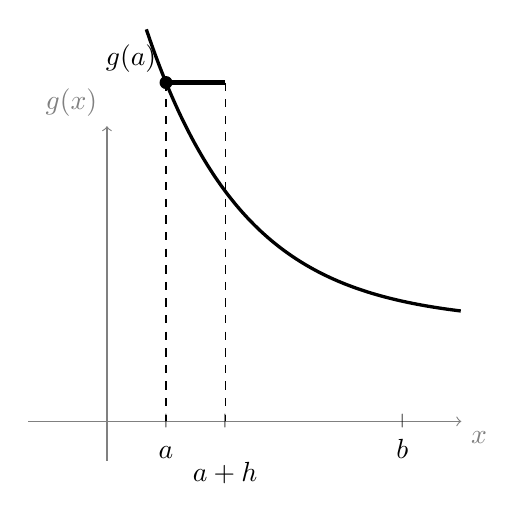
\begin{tikzpicture}[scale = 2.5]
		\draw[very thick, domain = 0.2:1.8, samples=200, smooth] plot (\x,{exp(-2*(\x-0.4)) + 0.5});
		\draw [gray, ->] (0,-0.2) -- (0,1.5) node [above left] {$g(x)$};
		\draw [gray, ->] (-0.4,0) -- (1.8,0) node [below right] {$x$};
		\draw [fill = black] (0.3, {exp(-2*(0.3-0.4)) + 0.5}) circle (0.03cm) node [above left] {$g(a)$};
		\draw [dashed] (0.3, {exp(-2*(0.3-0.4)) + 0.5}) -- (0.3,0);
		\draw [dashed] (0.6, {exp(-2*(0.3-0.4)) + 0.5}) -- (0.6,0);
		\draw [ultra thick] (0.3, {exp(-2*(0.3-0.4)) + 0.5}) -- (0.6, {exp(-2*(0.3-0.4)) + 0.5});
		\draw (0.3, 0) node {\tiny{$|$}} node [below = 2mm] {$a$};
		\draw (0.6, 0) node {\tiny{$|$}} node [below = 4mm] {$a + h$};
		\draw (1.5, 0) node {\tiny{$|$}} node [below = 1mm] {$b$};
		%\draw (2/3,0) node {$|$} node [above = 1mm] {$\alpha$};
	\end{tikzpicture}
\end{center}
We have approximated $g(x)$ from $a$ to $a+h$, by a single flat line. The area between this line and the $x$-axis is the area of a rectangle with side lengths $h$ (along the bottom) and $g(a)$ (up the side); the formula for the area of such a rectangle is Area $ = hg(a)$. Now, we can continue to approximate the remainder of $g(x)$ between $a$ and $b$: We find $g(a+h)$, and then multiply this by $h$, then we do the same for $g(a + 2h)$, and then $g(a + 3h)$, and so on, all the way to $b$:
\begin{center}
	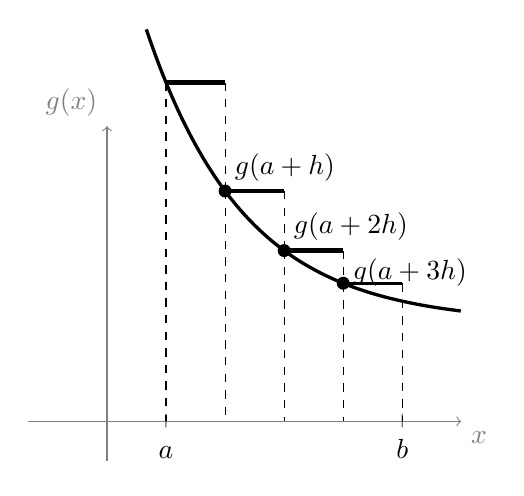
\begin{tikzpicture}[scale = 2.5]
		\draw[very thick, domain = 0.2:1.8, samples=200, smooth] plot (\x,{exp(-2*(\x-0.4)) + 0.5});
		\draw [gray, ->] (0,-0.2) -- (0,1.5) node [above left] {$g(x)$};
		\draw [gray, ->] (-0.4,0) -- (1.8,0) node [below right] {$x$};
		%\draw [fill = black] (0.3, {exp(-2*(0.3-0.4)) + 0.5}) circle (0.03cm) node [above left] 			        {$f(a)$};
		\draw (0.3, 0) node {\tiny{$|$}} node [below = 2mm] {$a$};
		%\draw (0.6, 0) node {\tiny{$|$}} node [below = 4mm] {$a + h$};
		\draw (1.5, 0) node {\tiny{$|$}} node [below = 1mm] {$b$};
		
		%first rectangle
		\draw [dashed] (0.3, {exp(-2*(0.3-0.4)) + 0.5}) -- (0.3,0);
		\draw [dashed] (0.6, {exp(-2*(0.3-0.4)) + 0.5}) -- (0.6,{exp(-2*(0.6-0.4)) + 0.5});
		\draw [ultra thick] (0.3, {exp(-2*(0.3-0.4)) + 0.5}) -- (0.6, {exp(-2*(0.3-0.4)) + 0.5});
		
		%second rectange
		\draw [fill = black] (0.6, {exp(-2*(0.6-0.4)) + 0.5}) circle (0.03cm) node [above right] 				{$g(a+h)$};
		\draw [dashed] (0.6, {exp(-2*(0.6-0.4)) + 0.5}) -- (0.6,0);
		\draw [dashed] (0.9, {exp(-2*(0.6-0.4)) + 0.5}) -- (0.9,{exp(-2*(0.9-0.4)) + 0.5});
		\draw [ultra thick] (0.6, {exp(-2*(0.6-0.4)) + 0.5}) -- (0.9, {exp(-2*(0.6-0.4)) + 0.5});
		
		%third
		\draw [fill = black] (0.9, {exp(-2*(0.9-0.4)) + 0.5}) circle (0.03cm) node [above right] 				{$g(a+2h)$};
		\draw [dashed] (0.9, {exp(-2*(0.9-0.4)) + 0.5}) -- (0.9,0);
		\draw [dashed] (1.2, {exp(-2*(0.9-0.4)) + 0.5}) -- (1.2,0);
		\draw [ultra thick] (0.9, {exp(-2*(0.9-0.4)) + 0.5}) -- (1.2, {exp(-2*(0.9-0.4)) + 0.5});
		
		%fourth
		\draw [fill = black] (1.2, {exp(-2*(1.2-0.4)) + 0.5}) circle (0.03cm);
		\draw [fill = black] (1.2, {exp(-2*(1.4-0.4)) + 0.5}) node [above right] 							{$g(a+3h)$};
		\draw [dashed] (1.2, {exp(-2*(1.2-0.4)) + 0.5}) -- (1.2, {exp(-2*(1.5-0.4)) + 0.5});
		\draw [dashed] (1.5, {exp(-2*(1.2-0.4)) + 0.5}) -- (1.5,0);
		\draw [very thick] (1.2, {exp(-2*(1.2-0.4)) + 0.5}) -- (1.5, {exp(-2*(1.2-0.4)) + 0.5});
	\end{tikzpicture}
\end{center}
So, summing up all of our rectangles we have
\[
hg(a) + hg(a+h) +  hg(a+2h) +  hg(a+3h).
\]
We can simplify it by factoring out the $h$ to get
\[
h\squac{g(a) + g(a+h) +  g(a+2h) +  g(a+3h)}
\]
We need to let $h$ get smaller (eventually infinitesimally small), since the smaller our choice for $h$, the more accurate the approximation becomes. As $h$ gets smaller, we need to create more rectangles in order to cover the distance from $a$ to $b$, so we need to add more terms to the sum. It is also convenient if we make sure that $h$ divides evenly into the distance $b - a$, so that the rectangles fit perfectly. So, we need to define $h$ as some fraction of the distance $b - a$. Hence we define
\[
h = \frac{b-a}{n}, \;\;\; \text{for some $n$}.
\]
Now, if we want $h$ to get infinitesimally small we just let $n \rightarrow \infty$. Our sum becomes,
\[
h\squac{g(a) + g(a+h) + g(a + 2h) + \ldots + g(a + nh)}, \;\;\; \text{where $n \rightarrow \infty$}
\]
Notice that since we defined $h$ so that $b - a$ is cut into $n$ pieces, it follows that we must have $n$ terms (i.e., $n$ rectangles) in our sum. Rewriting it in summation notation, we get
\[
h\sum_{k = 0}^n\brac{g(a+kh)}, \;\;\; \text{where $h = \frac{b-a}{n}$ and $n \rightarrow \infty$}
\]
Which we can take as the definition of the \textbf{integral from $\boldsymbol{a}$ to $\boldsymbol{b}$}. Using limit notation, we can write this as \label{integral}

  	\bigskip
	
	\hfil\fbox{
	\begin{minipage}{0.5\columnwidth}{
	
	%\vskip 0.05cm
	\begin{center}
	$\displaystyle{\int_a^b g(x) \; dx \; = \lim_{n \rightarrow \infty} \brac{h\sum_{k = 0}^n\brac{g(a+kh)}}}$, \bsk $\displaystyle{\text{where} \; h = \frac{b-a}{n}.}$
	\end{center}
	}
	\end{minipage}}
	\bigskip
	\bigskip

\noindent Sometimes this is referred to as the \textbf{definite integral} from $a$ to $b$ (as opposed to an \textbf{indefinite integral}). The variables $a$ and $b$ are called the \textbf{terminals} of the integral. We will talk about indefinite integrals during section \ref{FTC}. \label{terminals}

\subsection{Some important formulas for integrals} \label{integration}
Just like differentiation, \textbf{integration}, the act of taking an integral, is a \textit{linear} operation (see section \ref{linearity}); out of the following four properties (which are presented in the boxes as solutions), property (3) and (4) are equivalent to saying that integration is linear. \\

\noindent Considering that integrals represent areas under the graph, what do you expect the following to be equal to?
\begin{enumerate}
\item $\displaystyle{\int_a^b f(x) \; dx + \int_b^c f(x) \; dx}$, \;\;\; \text{where $c > b > a$}
\item $\displaystyle{\int_a^a f(x) \; dx}$
\item $\displaystyle{\int_a^b\brac{f(x) + g(x)} \; dx}$
\item $\displaystyle{\int_a^b kf(x) \; dx}, \;\;\; \text{where $k$ is some real constant.}$
\end{enumerate}
\bigskip

\noindent \textit{Solution to (1):} \\
Thinking about areas under the graph of $f(x)$, we have.
\[
\text{Area from $a$ to $b$} + \text{Area from $b$ to $c$} = \text{Area from $a$ to $c$}
\]
Hence,

  	\bigskip
	
	\hfil\fbox{
	\begin{minipage}{0.5\columnwidth}{
	
	%\vskip 0.05cm
	\begin{center}
	$\displaystyle{\int_a^b f(x) \; dx + \int_b^c f(x) \; dx = \int_a^c f(x) \; dx.}$
	\end{center}
	}
	\end{minipage}}
	\bigskip
	\bigskip

\noindent \textit{Solution to (2):} \\
The area under the graph from one point, $a$, to itself, must be $0$, since the distance from $a$ to $a$ is $a-a = 0$ (a rectangle with one side of length zero has no area). Hence

  	\bigskip
	
	\hfil\fbox{
	\begin{minipage}{0.25\columnwidth}{
	
	%\vskip 0.05cm
	\begin{center}
	$\displaystyle{\int_a^a f(x) \; dx = 0.}$
	\end{center}
	}
	\end{minipage}}
	\bigskip
	\bigskip


\noindent \textit{Solution to (3):} \\
For any point $a$ in the domain of $f$, we have $f(a) + g(a)$ is equal to the height, $f(a)$, plus the height, $g(a)$. Hence any point on the function $f(x) + g(x)$ will have a height equal to the the sum of the heights of both functions at that point. So
\[
\text{Area under $f(x) + g(x) = $ Area under $f(x) \;+\; $Area under $g(x)$}.
\]
Thus

  	\bigskip
	
	\hfil\fbox{
	\begin{minipage}{0.6\columnwidth}{
	
	%\vskip 0.05cm
	\begin{center}
	$\displaystyle{\int_a^b\brac{f(x) + g(x)}\; dx = \int_a^b f(x) \; dx + \int_a^b g(x) \; dx.}$
	\end{center}
	}
	\end{minipage}}
	\bigskip
	\bigskip


\noindent \textit{Solution to (4):} \\
For any point $a$ in the domain of $f$, we have $kf(a)$ is equal to the height, $f(a)$ multiplied by the constant, $k$. Hence,
\[
\text{Area under $kf(x) = k\times \brac{\text{Area under}\; f(x)}$}.
\]
So,

  	\bigskip
	
	\hfil\fbox{
	\begin{minipage}{0.45\columnwidth}{
	
	%\vskip 0.05cm
	\begin{center}
	$\displaystyle{\int_a^b\brac{kf(x)} \; dx = k\int_a^b\brac{f(x)} \; dx.}$
	\end{center}
	}
	\end{minipage}}
	\bigskip
	\bigskip
	
\subsection{An important definition} \label{integral b to a}
We have so far understood definite integrals to be the area under the graph along the interval $[a,b]$ where $a < b$ (this is the integral from $a$ to $b$). What about the integral from $b$ to $a$? When $a < b$, the interval $[b,a]$ doesn't make any sense, so we can't talk about the area under the graph. It turns out that a sensible definition for this integral is

  	\bigskip
	
	\hfil\fbox{
	\begin{minipage}{0.38\columnwidth}{
	
	%\vskip 0.05cm
	\begin{center}
	$\displaystyle{\int_b^a f(x) \; dx = -\int_a^b f(x) \; dx}$
	\end{center}
	}
	\end{minipage}}
	\bigskip
	\bigskip
	
\noindent So, we have just defined the integral from $b$ to $a$ to be the negative of the integral from $a$ to $b$. 

\section{Accumulation functions} \label{A(x)}
While doing probability, and particularly while finding the cumulative distribution function of a continuous random variable (which we will begin learning about in lecture 16), it will be useful for us to sum up all of the values that a function, $f(x)$, takes, up to a particular input value for $x$. \\

\noindent Suppose that we have some starting point $x = a$, and we wish to define a function, say $A(x)$, which integrates $f(x)$, from $a$, along to some arbitrary point, $x$. Then we can define

  	\bigskip
	
	\hfil\fbox{
	\begin{minipage}{0.3\columnwidth}{
	
	%\vskip 0.05cm
	\begin{center}
	$\displaystyle{A(x) = \int_a^x f(t) \; dt.}$
	\end{center}
	}
	\end{minipage}}
	\bigskip
	\bigskip

\noindent We are still integrating the function $f(x)$, but we have replaced the dummy variable, $x$, from the integral, with another dummy variable, $t$. The reason we do this is that we do not want to confuse the variable that we are integrating \textit{along} to (which we have labelled $x$), with the variable that we are integrating \textit{with respect} to (which we have labelled $t$). We call $A(x)$ the \textbf{accumulation function}. \\

\noindent For example, \\
\begin{center}
	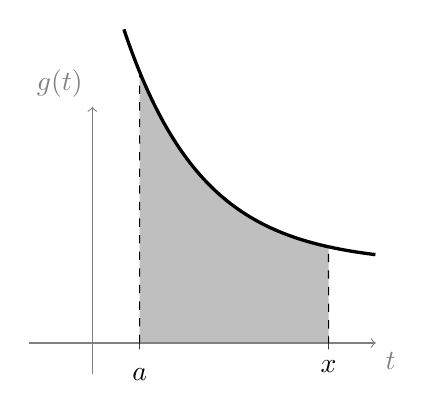
\begin{tikzpicture}[scale = 2]
		\draw [dashed, fill=gray!50, domain = 0.3:1.5, samples=200, smooth] (0.3,0) -- plot (\x,{exp(-2*(\x-0.4)) + 0.5}) -- (1.5,0);
		\draw [very thick, domain = 0.2:1.8, samples=200, smooth] plot (\x,{exp(-2*(\x-0.4)) + 0.5});
		\draw [gray, ->] (0,-0.2) -- (0,1.5) node [above left] {$g(t)$};
		\draw [gray, ->] (-0.4,0) -- (1.8,0) node [below right] {$t$};
		\draw (0.3, 0) node {\tiny{$|$}} node [below = 2mm] {$a$};
		\draw (1.5, 0) node {\tiny{$|$}} node [below = 1mm] {$x$};
		%\draw (0.3,0) -- (0.3,{exp(-2*(0.3-0.4)) + 0.5});
		%\draw (2/3,0) node {$|$} node [above = 1mm] {$\alpha$};
	\end{tikzpicture}
\end{center}
The grey area under the above graph depicts

\[
\int_a^x g(t) \; dt.
\]

\noindent Recall (from section \ref{cdf}) that the cumulative distribution function, $F(x)$, of a random variable, $X$, is defined to be $F(x) = P(X \leq x)$. When $X$ is discrete, we found that $F(x)$ is the sum of the individual probabilities associated with every value that $X$ takes, up to and including $x$. That is, $F(x)$ considers all possible values that $X$ takes within the interval $(-\infty,x].$ When we begin to find cumulative distribution functions for \textit{continuous} random variables, we will again be concerned with summing up every value that a random variable takes in the interval $(-\infty,x].$ \\

\noindent If we wish to define a function, $F(x)$, that gives us a running total of every value that a continuous function, $f(x)$, takes, from $-\infty$ along to $x$, then we can use the same formula that we had for $A(x)$, but we let $a \rightarrow -\infty$. So we get,

  	\bigskip
	
	\hfil\fbox{
	\begin{minipage}{0.3\columnwidth}{
	
	%\vskip 0.05cm
	\begin{center}
	$\displaystyle{F(x) = \int_{-\infty}^x f(t) \; dt.}$
	\end{center}
	}
	\end{minipage}}
	\bigskip
	\bigskip

\noindent Sometimes this function is also referred to as $A(x)$. On the graph of a bell curve, this area might appear as follows:
\begin{center}
	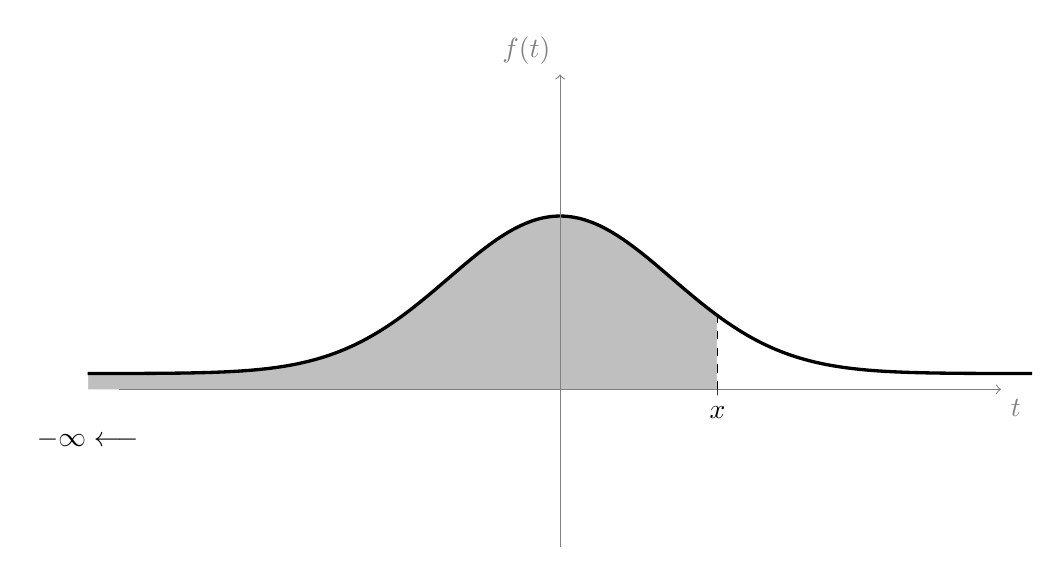
\begin{tikzpicture} [scale = 2]
	\draw[white, fill = gray!50, domain = -3:1, samples=200, smooth] (-3,0)  -- plot (\x,{exp(-(\x)^2) + 0.1}) -- (1,0);
	\draw [dashed] (1,0) -- (1,{exp(-(1)^2) + 0.1});
	\draw[very thick, domain = -3:3, samples=200, smooth] plot (\x,{exp(-(\x)^2) + 0.1});
	\draw [gray, ->] (0,-1) -- (0,2) node [above left] {$f(t)$};
	\draw [gray, ->] (-2.8,0) -- (2.8,0) node [below right] {$t$};
	\draw (-3,0) [below = 2mm] node {$-\infty \longleftarrow$};
	\draw (1,0) node {\tiny{$|$}} node [below = 1mm] {$x$};
	\end{tikzpicture}
\end{center}

\noindent Integrals that have one or both terminals replaced by $-\infty$ or $\infty$ are called \textbf{improper integrals}. Improper integrals are still a type of definite integral. \label{improper integral}

\subsection{Fundamental theorem of calculus} \label{FTC} \label{indefinite integral}
The fundamental theorem of calculus (FTC) is a two part theorem which deals with the relationship between \textit{rate of change} (differentiation) and \textit{area under a curve} (integration). \\

\noindent Before we state the FTC, we need to start by defining the idea of \textbf{antidifferentiation}, as a process which \textit{undoes} the action of taking the derivative. In other words, for some function $f(x)$, we define an \textbf{antiderivative} of $f(x)$ to be a function, $\mathcal{F}(x)$, whose derivative is $f(x)$. \\

\noindent As an example, we can find an antiderivative of the function $f(x) = 2x$, by recognising that $2x$ is the derivative of $x^2$. So, $x^2$ is an antiderivative of $2x$. That is, $\mathcal{F}(x) = x^2$. \\

\noindent Why have we referred to $x^2$ as \textit{an} antiderivative of $f(x)$, rather than \textit{the} antiderivative of $f(x)$? The answer is that our definition of antiderivative allows there to be more than one antiderivative of $2x$. The function $x^2 + c$, where $c$ is any real constant, has derivative $\frac{d}{dx}\brac{x^2 + c} = \frac{d}{dx}\brac{x^2} + \frac{d}{dx}\brac{c} = 2x + 0 = 2x$. Hence, $f(x) = 2x$ has an infinite number of antiderivatives of the form $\mathcal{F}(x) = x^2 + c$, since there are an infinite number of choices for the constant, $c$. This is true in general for all functions that have an antiderivative. The constant, $c$, is sometimes referred to as the \textbf{constant of integration}.  \label{constant of integration} \\


\subsubsection{First part}
\noindent The antiderivative also goes by the name, \textbf{indefinite integral}. The first part of the fundamental theorem of calculus (given here without proof) tells us exactly how an antiderivative is related to the definite integral. Let $\mathcal{F}(x)$ be an antiderivative of some (continuous) function, $f(x)$. Then \textbf{the first part of the fundamental theorem of calculus says that}

  	\bigskip
	
	\hfil\fbox{
	\begin{minipage}{0.45\columnwidth}{
	
	%\vskip 0.05cm
	\begin{center}
	$\displaystyle{\int_a^b f(x) \; dx = \mathcal{F}(b) - \mathcal{F}(a).}$
	\end{center}
	}
	\end{minipage}}
	\bigskip
	\bigskip


\noindent On the left we have the definite integral from $a$ to $b$, and on the right we have the difference of an antiderivate of $f$, evaluated at $b$, from that evaluated at $a$.  \\

\noindent Soon we will use this fact to find definite integrals, using some formulas that we will develop for common antiderivatives. Note that, while $f(x)$ has infinitely many antiderivatives, a particular definite integral is always unique (hence the word, ``definite''). \\

\noindent An alternative way to write the first part of the FTC is
\[
\int_a^b \frac{d}{dx}\brac{f(x)} \; dx = f(b) - f(a).
\]

\subsubsection{Second part}
We have already defined antidifferentiation so that it is inverse to differentiation. It follows that differentiation undoes antidifferentiation (just as antidifferentiation undoes diffetentiation).  \textbf{The second part of the fundamental theorem of calculus} takes this one step further. It states that differentiation also undoes the \textit{accumulation function}, $F(x)$. In other words, if we have a function, $f(x)$, that is defined on some interval $[a,b]$, then

  	\bigskip
	
	\hfil\fbox{
	\begin{minipage}{0.45\columnwidth}{
	
	%\vskip 0.05cm
	\begin{center}
	$\displaystyle{\frac{d}{dx}\brac{\int_a^xf(t) \; dt}} = f(x)$
	\end{center}
	}
	\end{minipage}}
	\bigskip
	\bigskip

\noindent Notice that the function inside the brackets is the accumulation function from section \ref{A(x)}. This means that, conveniently, the accumulation function is itself an antiderivative; this completes the picture, finishing the job of showing how definite integrals are related to antiderivatives. A definite integral can be specified in terms of an antiderivative (part 1), and the accumulation function (a type of definite integral) is a particular antiderivative. \\

\noindent If the function, $f(x)$, has the entire set of real numbers as its domain, then we would replace $a$ with $-\infty$; thus writing the second part as
\[
\frac{d}{dx}\brac{\int_{-\infty}^xf(t) \;dt} = f(x).
\]

\section{Finding antiderivatives} \label{derivativetable1}
We can find antiderivatives by working backwards from known derivatives. In sections \ref{derivative formulas} and \ref{more derivative formulas} we developed the derivatives in the following table:
\begin{center}
$\begin{array}{|c|c|c|} \hline
 \boldsymbol{f(x)} 			& \boldsymbol{f'(x)} 		& \textbf{Comments} \\ \hline
g(x) + h(x)	& g'(x) + h'(x)   & \text{sum} \\
cg(x)			& cg'(x)		& c \; \text{constant} \\ \hline
c 			& 0 			& c \; \text{constant} \\ \hline
x^k			& kx^{k-1} 	& k \neq 0	  	      	\\ \hline
\e^{ax}		&a\e^{ax} 	&				\\ \hline
\log_e(x)		&\frac{1}{x}	& x > 0			\\ \hline
\end{array}$
\end{center}

\subsubsection{Powers}
We wish to find an antiderivative of $f(x) = x^k$. That is, we want to find a function, $\mathcal{F}(x)$, whose derivative is $\mathcal{F}'(x) = x^k$. \\

\noindent Since $x^k$ is a power function, we will assume the antiderivative is of the form $\mathcal{F}(x)~=~ax^b$, for some real numbers $a,b$ with $b \neq 0$ (which is the general form of a power function). We know from the above table that the derivative of $ax^b$ is $abx^{b-1}$. So $\mathcal{F}'(x)~=~abx^{b-1}$. Hence, we require $abx^{b-1} = x^k$. Comparing $abx^{b-1}$ to $x^k$, we can see that we need
\[
(1) \;\; ab = 1 \qquad \text{and} \qquad (2) \;\; b-1 = k.
\]
Rearranging $b-1 = k$ gives $b = k + 1$. Substituting $b = k + 1$ into equation (1) gives $a(k+1) = 1$; dividing both sides of this by $k+1$ gives $a = \frac{1}{k+1}$. Now we know that $a = \frac{1}{k+1}$ and $b = k + 1$. Hence
\[
\mathcal{F}(x) = ax^b = \frac{1}{k+1}x^{k+1}
\] 
There is one important thing to note here. We have divided by a variable, $k+1$. So, we cannot have $k + 1 = 0$, i.e., we cannot have $k = -1$.
Thus,

  	\bigskip
	
	\hfil\fbox{
	\begin{minipage}{0.9\columnwidth}{
	
	%\vskip 0.05cm
	\begin{center}
	$f(x) = x^k$ \;\; implies \;\; $\mathcal{F}(x) = \frac{1}{k+1}x^{k+1}$ \;\; is an antiderivative (where $k \neq -1$)
	\end{center}
	}
	\end{minipage}}
	\bigskip
	\bigskip
	
\noindent When $k = -1$ we have $x^k = x^{-1} = \frac{1}{x}$ which is a case that we will deal with separately.

\subsubsection{Constants}
We wish to find an antiderivative of $f(x) = c$, where $c$ is some real constant. With some thought and experience, we can try the function $\mathcal{F}(x) = cx$. Then,
\[
\mathcal{F}'(x) = \frac{d}{dx}\brac{cx} = c\frac{d}{dx}\brac{x^1} = cx^{1-1} = cx^0 = c.
\]
So we can conclude that
%So, we want a function, $\mathcal{F}(x)$, whose derivative is $c$. Again, we look for a function of the form $\mathcal{F}(x) = ax^b$ (a power function). Again we have $\mathcal{F'(x)} = abx^{b-1}$. So we require $abx^{b-1} = c$. \\
%
%Comparing $abx^{b-1}$ with $c$, we can see that we need to get rid of the variable, $x$. If $b - 1 = 0$, then $x^{b-1} = x^0 = 1$; this is the only way that we can make $x^{b-1}$ remain constant, since all other powers of $x$ are non-constant. Hence we we know that $b-1 = 0$; rearranging gives $b = 1$. So substituting $b = 1$ into $abx^{b-1}$ we can see that
%\[
%c = ax^{1-1} = ax^0 = a.
%\]    
%So we must have $a = c$ and $b = 1$. Hence
%\[
%\mathcal(F)(x) = ax^b = cx^1 = cx.
%\]

  	\bigskip
	
	\hfil\fbox{
	\begin{minipage}{0.7\columnwidth}{
	
	%\vskip 0.05cm
	\begin{center}
	$f(x) = c$ \;\; implies \;\; $\mathcal{F}(x) = cx$ \;\; is an antiderivative
	\end{center}
	}
	\end{minipage}}
	\bigskip
	\bigskip

\subsubsection{Exponentials}
We want an antiderivative of $f(x) = \e^{ax}$, where $a$ is a real constant. We could find this algebraically (like we did with powers) but instead we will just make a guess and see if it works (like we did with constants); both methods can be very useful. We know that the derivative of $\e^{ax}$ is $a\e^{ax}$, so let's try $\mathcal{F}(x) = \frac{1}{a}\e^{ax}$. Then
\[
\mathcal{F}'(x) = \frac{d}{dx}\brac{\frac{1}{a}\e^{ax}} = \frac{1}{a}\frac{d}{dx}\brac{\e^{ax}} = \frac{1}{a}\brac{a\e^{ax}} = \e^{ax}.
\]
So

  	\bigskip
	
	\hfil\fbox{
	\begin{minipage}{0.7\columnwidth}{
	
	%\vskip 0.05cm
	\begin{center}
	$f(x) = \e^{ax}$ \;\; implies \;\; $\mathcal{F}(x) = \frac{1}{a}\e^{ax}$ \;\; is an antiderivative
	\end{center}
	}
	\end{minipage}}
	\bigskip
	\bigskip

\subsubsection{Power with $\boldsymbol{k = -1}$ (i.e., $\boldsymbol{f(x) = \frac{1}{x}}$)}
From our table of derivates we can see that the derivative of $\ln(x)$ is $\frac{1}{x}$. This means we are done! It follows that an antiderivative of $\frac{1}{x}$ is $\ln(x)$. \\

\noindent We do need to be careful to note that the domain of $\ln(x)$ is $x > 0$, while the domain of $\frac{1}{x}$ is all real numbers except $0$. To deal with this problem, we sometimes say that the antiderivative of $\frac{1}{x}$ is $\ln(|x|)$, where the absolute value function maps negative values of $x$ to positive ones. However, for our purposes it is sufficient to restrict the domain of $\frac{1}{x}$ to $x > 0$. So,

  	\bigskip
	
	\hfil\fbox{
	\begin{minipage}{0.85\columnwidth}{
	
	%\vskip 0.05cm
	\begin{center}
	$f(x) = \frac{1}{x}$ \;\; implies \;\; $\mathcal{F}(x) = \ln(x)$ \;\; is an antiderivative (where $x > 0$)
	\end{center}
	}
	\end{minipage}}
	\bigskip
	\bigskip

\subsubsection{Summary}

\begin{center}
$\begin{array}{|c|c|c|} \hline
 \boldsymbol{f(x)} & \boldsymbol{\mathcal{F}(x)} & \textbf{Comments} \\ \hline
x^k				& \frac{1}{k+1}x^{k+1} 	& k \neq 1 \\ \hline
\e^{ax}			& \frac{1}{a}\e^{ax}		& a \; \text{constant}\\ \hline
c 				& cx 						& c \; \text{constant} \\ \hline
\frac{1}{x}		& \ln(x) 					& x > 0	  	      \\	\hline
\end{array}$
\end{center}
In section \ref{integration} we mentioned that definite integrals are linear. The same holds for antiderivatives; that is, the sum formula, and constant multiples formula, both hold for antiderivatives as well.

\subsection{Some notation for antiderivatives} \label{symbindefiniteintegral}
Antiderivatives (also known as indefinite integrals) have their own notation similar to the one we use for definite integrals. We write

  	\bigskip
	
	\hfil\fbox{
	\begin{minipage}{0.35\columnwidth}{
	
	%\vskip 0.05cm
	\begin{center}
	$\displaystyle{\mathcal{F}(x) = \int f(x) \; dx}$
	\end{center}
	}
	\end{minipage}}
	\bigskip
	\bigskip

\noindent This is just like the notation for a definite integral, but the terminals have been left off to reflect the fact that there are an infinite number of antiderivatives for any particular $f(x)$ (corresponding to an infinite number of possible choices for the constant (see section \ref{FTC})).

\subsection{Example}
Find antiderivatives of the following expressions,
\begin{enumerate}
\item $\e^{-6x} + 4x^{-3} + 7$, \;\;\; where $x \neq 0$
\item $x^4 + 2x^{-1} + \sqrt{x}$, \;\;\; where $x > 0$
\item $x(x^3 - 2x^{-1})$
\end{enumerate}
In each case you could add a constant of integration, $c$, to your expression for the antiderivative, but we will leave the constant out (i.e., we have $c = 0$).

\noindent \textit{Solution to (1):} \\
\begin{align*}
\int \e^{-6x} + 4x^{-3} + 7 \; dx & =  \int \e^{-6x} \; dx + 4\int x^{-3} \; dx + \int 7 \; dx \tag{linearity} \\
	& = -\frac{1}{6}\e^{6x} + \frac{4}{-3+1}x^{-3+1} + 7x \tag{antiderivative formulas} \\
	& = -\frac{1}{6}\e^{6x} - \frac{4}{2}x^{-2} + 7x.
\end{align*}

\noindent \textit{Solution to (2):} \\
\begin{align*}
\int x^4 + 2x^{-1} + \sqrt{x} \; dx & =  \int x^4 \; dx + 2\int x^{-1} \; dx + \int x^{1/2} \; dx \tag{linearity} \\
 		& = \frac{1}{4+1}x^{4+1} + 2\ln(x) + \frac{1}{1/2+1}x^{1/2+1} \tag{formulas}  \\
 		& = \frac{1}{5}x^5 + 2\ln(x) + \frac{2}{3}x^{3/2}.
\end{align*}

\noindent \textit{Solution to (3):} \\
\begin{align*}
\int x(x^3 - 2x^{-1}) \; dx & = \int x^4 - 2 \; dx \tag{expanding brackets} \\
	& = \int x^4 \; dx - \int 2 \; dx \\
	& = \frac{1}{5}x^5 - 2x \tag{formulas}
\end{align*}



\section{Using FTC to find definite integrals} \label{Using FTC to find definite integrals}
Recall from section \ref{FTC} that the first part of the fundamental theorem of calculus says that we can find definite integrals in terms of (a difference of) indefinite integrals (i.e., antiderivatives). That is, 
\[
\int_a^b f(x) \; dx = \mathcal{F}(b) - \mathcal{F}(a).
\]
Where $\mathcal{F}(x)$ is an antiderivative, i.e.,
\[
\mathcal{F}(x) = \int f(x) \; dx. \tag{$\bigstar$}
\]
Notice, as a side note, that if your antiderivative has some constant of integration, $c$, then it will cancel since $(\mathcal{F}(b) + c) - (\mathcal{F}(a) + c) =  \mathcal{F}(b) - \mathcal{F}(a)$. \\

\noindent Sometimes, to save space, we write, instead of $\mathcal{F}(b) - \mathcal{F}(a)$,
\[
\mathcal{F}(x)\big|_a^b \qquad \text{or} \qquad \squac{\mathcal{F}(x)}_a^b = \mathcal{F}(b) - \mathcal{F}(a)
\]
This means that we evaluate $\mathcal{F}(x)$ at $x = b$, and at $x = a$, then subtract the latter from the former. When one of the terminals, $a$ or $b$, is equal to $\infty$ or $-\infty$, this signifies that we want to take a limit. That is, for example,
\[
\mathcal{F}(x)\big|_\infty^b =  \mathcal{F}(b) - \lim_{a \rightarrow \infty}\brac{\mathcal{F}(a)}
\]
If we want, we can rewrite this as (because of ($\bigstar$)) 
\[
\mathcal{F}(x)\big|_\infty^b = \int f(b) \; dx - \lim_{a \rightarrow \infty}\brac{ \int f(a) \; dx}
\]
We will look at how this notation is used in practice in the next two examples.
\subsection{Example}
Calculate the following definite integral
\[
\int_1^\infty \e^{-2x} \; dx 
\]

\noindent \textit{Solution:} \\
\begin{align*}
\int_1^\infty \e^{-2x} \; dx
		& = \squac{\int \e^{-2x} \; dx}_1^\infty \tag{by FTC} \\
		& = \squac{-\frac{1}{2}\e^{-2x}}_1^\infty \tag{antiderivative formulas} \\
		& = \lim_{b \rightarrow \infty}\brac{-\frac{1}{2}\e^{-2b}} - \brac{-\frac{1}{2}\e^{-2\times1}} \\
		& = 0 - \brac{-\frac{1}{2}\e^{-2}} \tag{since $e^{-2b} \rightarrow 0$ as $b \rightarrow \infty$} \\
		& = \frac{1}{2}\e^{-2}
\end{align*}
To clarify: $\e^{-2b} = \frac{1}{\e^{2b}}$; so, as $b \rightarrow \infty$ the denominator grows and the expression keeps getting smaller, i.e., $\e^{-2b} \rightarrow 0$.

\subsection{Example}
In practice you don't need to specifically write down that you are taking the limit, as long as you can safely see what the limit is (this is ok since most of the limits we will do in this subject are reasonably straight forward). For example: \\

\noindent Calculate the following definite integral
\[
\int_1^\infty \e^{-\frac{1}{2}x} + 2x^{-3} \; dx 
\]

\noindent \textit{Solution:} \\
\begin{align*}
\int_1^\infty \e^{-\frac{1}{2}x} + 2x^{-3} \; dx  & = \int_1^\infty \e^{-\frac{1}{2}x} \; dx +  2\int_1^\infty x^{-3} \; dx  \tag{linearity} \\
	& =  \squac{\int \e^{-\frac{1}{2}x} \; dx}_1^\infty +  2\squac{\int x^{-3} \; dx}_1^\infty \tag{FTC} \\
	& =  \squac{-2\e^{-\frac{1}{2}x}}_1^\infty +  2\squac{-\frac{1}{2} x^{-2}}_1^\infty \tag{integral formulas} \\
	& = 0 - \brac{-2\e^{-\frac{1}{2}\times1}} + 0 - 2\brac{-\frac{1}{2}1^{-2}} \tag{both $0$ are due to limits} \\
	& = 2\e^{-\frac{1}{2}} + 1.
\end{align*}

\subsection{Example} \label{ex13.1}
Sketch this function, and then find $A(x)$ (the accumulation function) and the total area under the graph.
\[
f(x) = \left\{
  \begin{array}{ll}
    0, & \text{if} \; x \leq 1 \smallskip \\
    x - 1, & \text{if} \; 1 < x \leq 2 \smallskip \\
    3 - x, & \text{if} \; 2 < x \leq 3 \smallskip \\
    0,& \text{if} \; x > 3.
  \end{array}
\right.
\]

\noindent \textit{Solution:} \\
Sketch of $f(x)$
\begin{center}
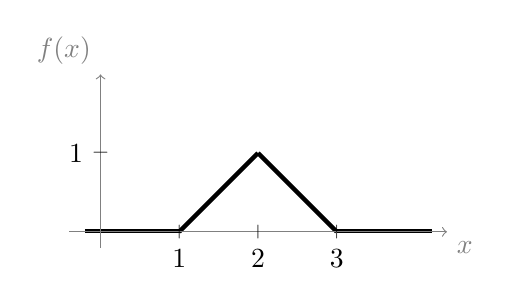
\begin{tikzpicture}
		\draw [ultra thick, fill=gray!50, domain = -0.2:1, samples=200, smooth] plot (\x,{0.01});
		\draw [ultra thick, fill=gray!50, domain = 1:2, samples=200, smooth] plot (\x,{\x-1});
		\draw [ultra thick, fill=gray!50, domain = 2:3, samples=200, smooth] plot (\x,{3-\x});
		\draw [ultra thick, fill=gray!50, domain = 3:4.2, samples=200, smooth] plot (\x,{0.01});
		\draw [gray, ->] (0,-0.2) -- (0,2) node [above left] {$f(x)$};
		\draw [gray, ->] (-0.4,0) -- (4.4,0) node [below right] {$x$};
		\draw (1,0) node {\tiny{$|$}} node [below = 1mm] {$1$};
		\draw (2,0) node {\tiny{$|$}} node [below = 1mm] {$2$};
		\draw (3,0) node {\tiny{$|$}} node [below = 1mm] {$3$};
		\draw (0,1) node [rotate = -90] {\tiny{$|$}} node [left = 1mm] {$1$};
\end{tikzpicture}
\end{center}

\noindent From section \ref{A(x)}, the accumulation function is
\[
A(x) = \int_{-\infty}^x f(t) \; dt
\]
Since $f(x)$ is defined differently for different sections of its domain, we will need to do the same for $A(x)$. \\
\textbf{For $\boldsymbol{x \leq 1}$:}
\begin{align*}
A(x)  & = \int_{-\infty}^1 0 \; dt  \\
	& = 0.
\end{align*}
\textbf{For $\boldsymbol{1 < x \leq 2}$:}
\begin{align*}
A(x)  & =  \int_{-\infty}^1 0 \; dt + \int_{1}^x t - 1 \; dt  \tag{since $f(x) = x-1$ when $x \in (1,2]$}\\
	& = 0 +  \int_{1}^x t \; dt - \int_1^x 1 \; dt \tag{linearity} \\
	& = \squac{\frac{1}{2}t^2}_1^x - \squac{t}_1^x \tag{FTC, and integral formulas} \\
	& = \frac{1}{2}x^2 - \frac{1}{2}1^2 - \brac{x - 1} \\
	& = \frac{1}{2}x^2 - x + \frac{1}{2}. \tag{$\star$}
\end{align*}
\textbf{For $\boldsymbol{2 < x \leq 3}$:}
\begin{align*}
A(x)  & =  \int_{-\infty}^1 0 \; dt + \int_{1}^2 t - 1 \; dt + \int_2^x 3-t \; dt \tag{since $f(x) = 3-x$ when $x \in (2,3]$} \\
	& = \frac{1}{2}(2)^2 - 2 + \frac{1}{2} + \int_2^x 3-t \; dt \tag{substituting $x = 2$ into ($\star$)} \\
	& = \frac{1}{2} + \int_2^x 3 \; dt - \int_2^x t \; dt \tag{linearity} \\
	& = \frac{1}{2} + \squac{3t}_2^x - \squac{\frac{1}{2}t^2}^x_2 \tag{FTC, and integral formulas} \\
	& = \frac{1}{2} + 3x - 3\times2 - \brac{\frac{1}{2}x^2 - \frac{1}{2}2^2} \\
	& = -\frac{1}{2}x^2 + 3x - \frac{7}{2}. \tag{$\dagger$}
\end{align*}
\textbf{For $\boldsymbol{x > 3}$:}
\begin{align*}
A(x)  & =  \int_{-\infty}^1 0 \; dt + \int_{1}^2 t - 1 \; dt + \int_2^3 3-t \; dt + \int_3^x 0 \; dt \tag{since $f(x) = 0$ when $x > 3$} \\
	& = - \frac{1}{2}3^2 + 3\times3 - \frac{7}{2} + 0 \tag{substituting $x = 3$ into ($\dagger$)} \\
	& = 1.
\end{align*}
\textbf{Putting all of our results together we get:}
\[
A(x) = \left\{
  \begin{array}{ll}
    0, & \text{if} \; x \leq 1 \smallskip \\
    \frac{1}{2}x^2 - x + \frac{1}{2}, & \text{if} \; 1 < x \leq 2 \smallskip \\
    -\frac{1}{2}x^2 + 3x - \frac{7}{2}, & \text{if} \; 2 < x \leq 3 \smallskip \\
    1,& \text{if} \; x > 3.
  \end{array}
\right.
\]